\section{Dataset}
This section provides an overview of the CASIA Multi-Spectral Palmprint Image Database, including data acquisition details and a description of the dataset.

\subsection{Data Aquisition}

The self-designed imaging device for acquiring hand images \cite{hao2008multispectral,hao2007comparative} is shown in Figure \ref{fig:device_architecture}. The device operates in a contact-free environment, The imaging process involves the following steps:

\begin{enumerate}
    \item \textbf{Illumination Setup}: The device uses six groups of LEDs (violet to near-infrared) activated sequentially, employing a time-division strategy to acquire multispectral images under varying illumination, capturing different skin layers through light absorption and scattering. 
    \item \textbf{Reflective Imaging}: Images are captured reflectively in a sheltered environment with consistent illumination, while circularly arranged LED groups, diffused with ground glass, ensure even lighting across the hand. 
    \item \textbf{Contact-Free Operation}: Subjects are instructed to naturally stretch their hands, palms facing the camera, without any physical contact with a tangible surface or plate. 
    \item \textbf{Sequential Image Capture}: A single camera is used to sequentially capture images under each spectral light. This time-division strategy improves scalability and offers a better performance-to-cost ratio compared to frequency-division methods requiring multiple cameras.
\end{enumerate}

\begin{figure}[H]
    \centering
    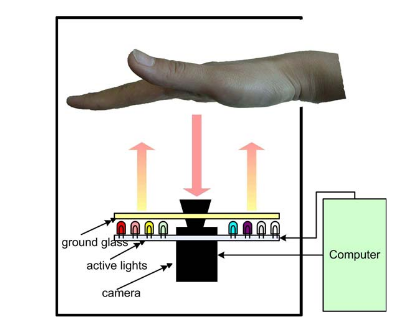
\includegraphics[width=0.3\textwidth]{./images/device-architecture.png}
    \caption{Device architecture for acquiring multispectral palm images.}
    \label{fig:device_architecture}
\end{figure}

\subsection{Dataset Description}

The CASIA Multi-Spectral Palmprint Image Database consists of 7,200 palm images captured from 100 individuals using a self-designed multispectral imaging device. The images are 8-bit gray-level JPEG files. For each hand, two sessions of palm images were captured, with a time interval of more than one month between the sessions to simulate real-world conditions and introduce natural variability. Each session includes three samples, with each sample containing six palm images captured simultaneously under six different electromagnetic spectrums, corresponding to wavelengths of 460 nm, 630 nm, 700 nm, 850 nm, 940 nm, and white light shown in Figure \ref{fig:dataset_example}. Variations in hand postures were allowed between the two sessions to increase the diversity of intra-class samples, thereby simulating practical usage scenarios and enhancing the robustness of biometric recognition systems trained on this dataset.

\begin{figure}[H]
    \centering
    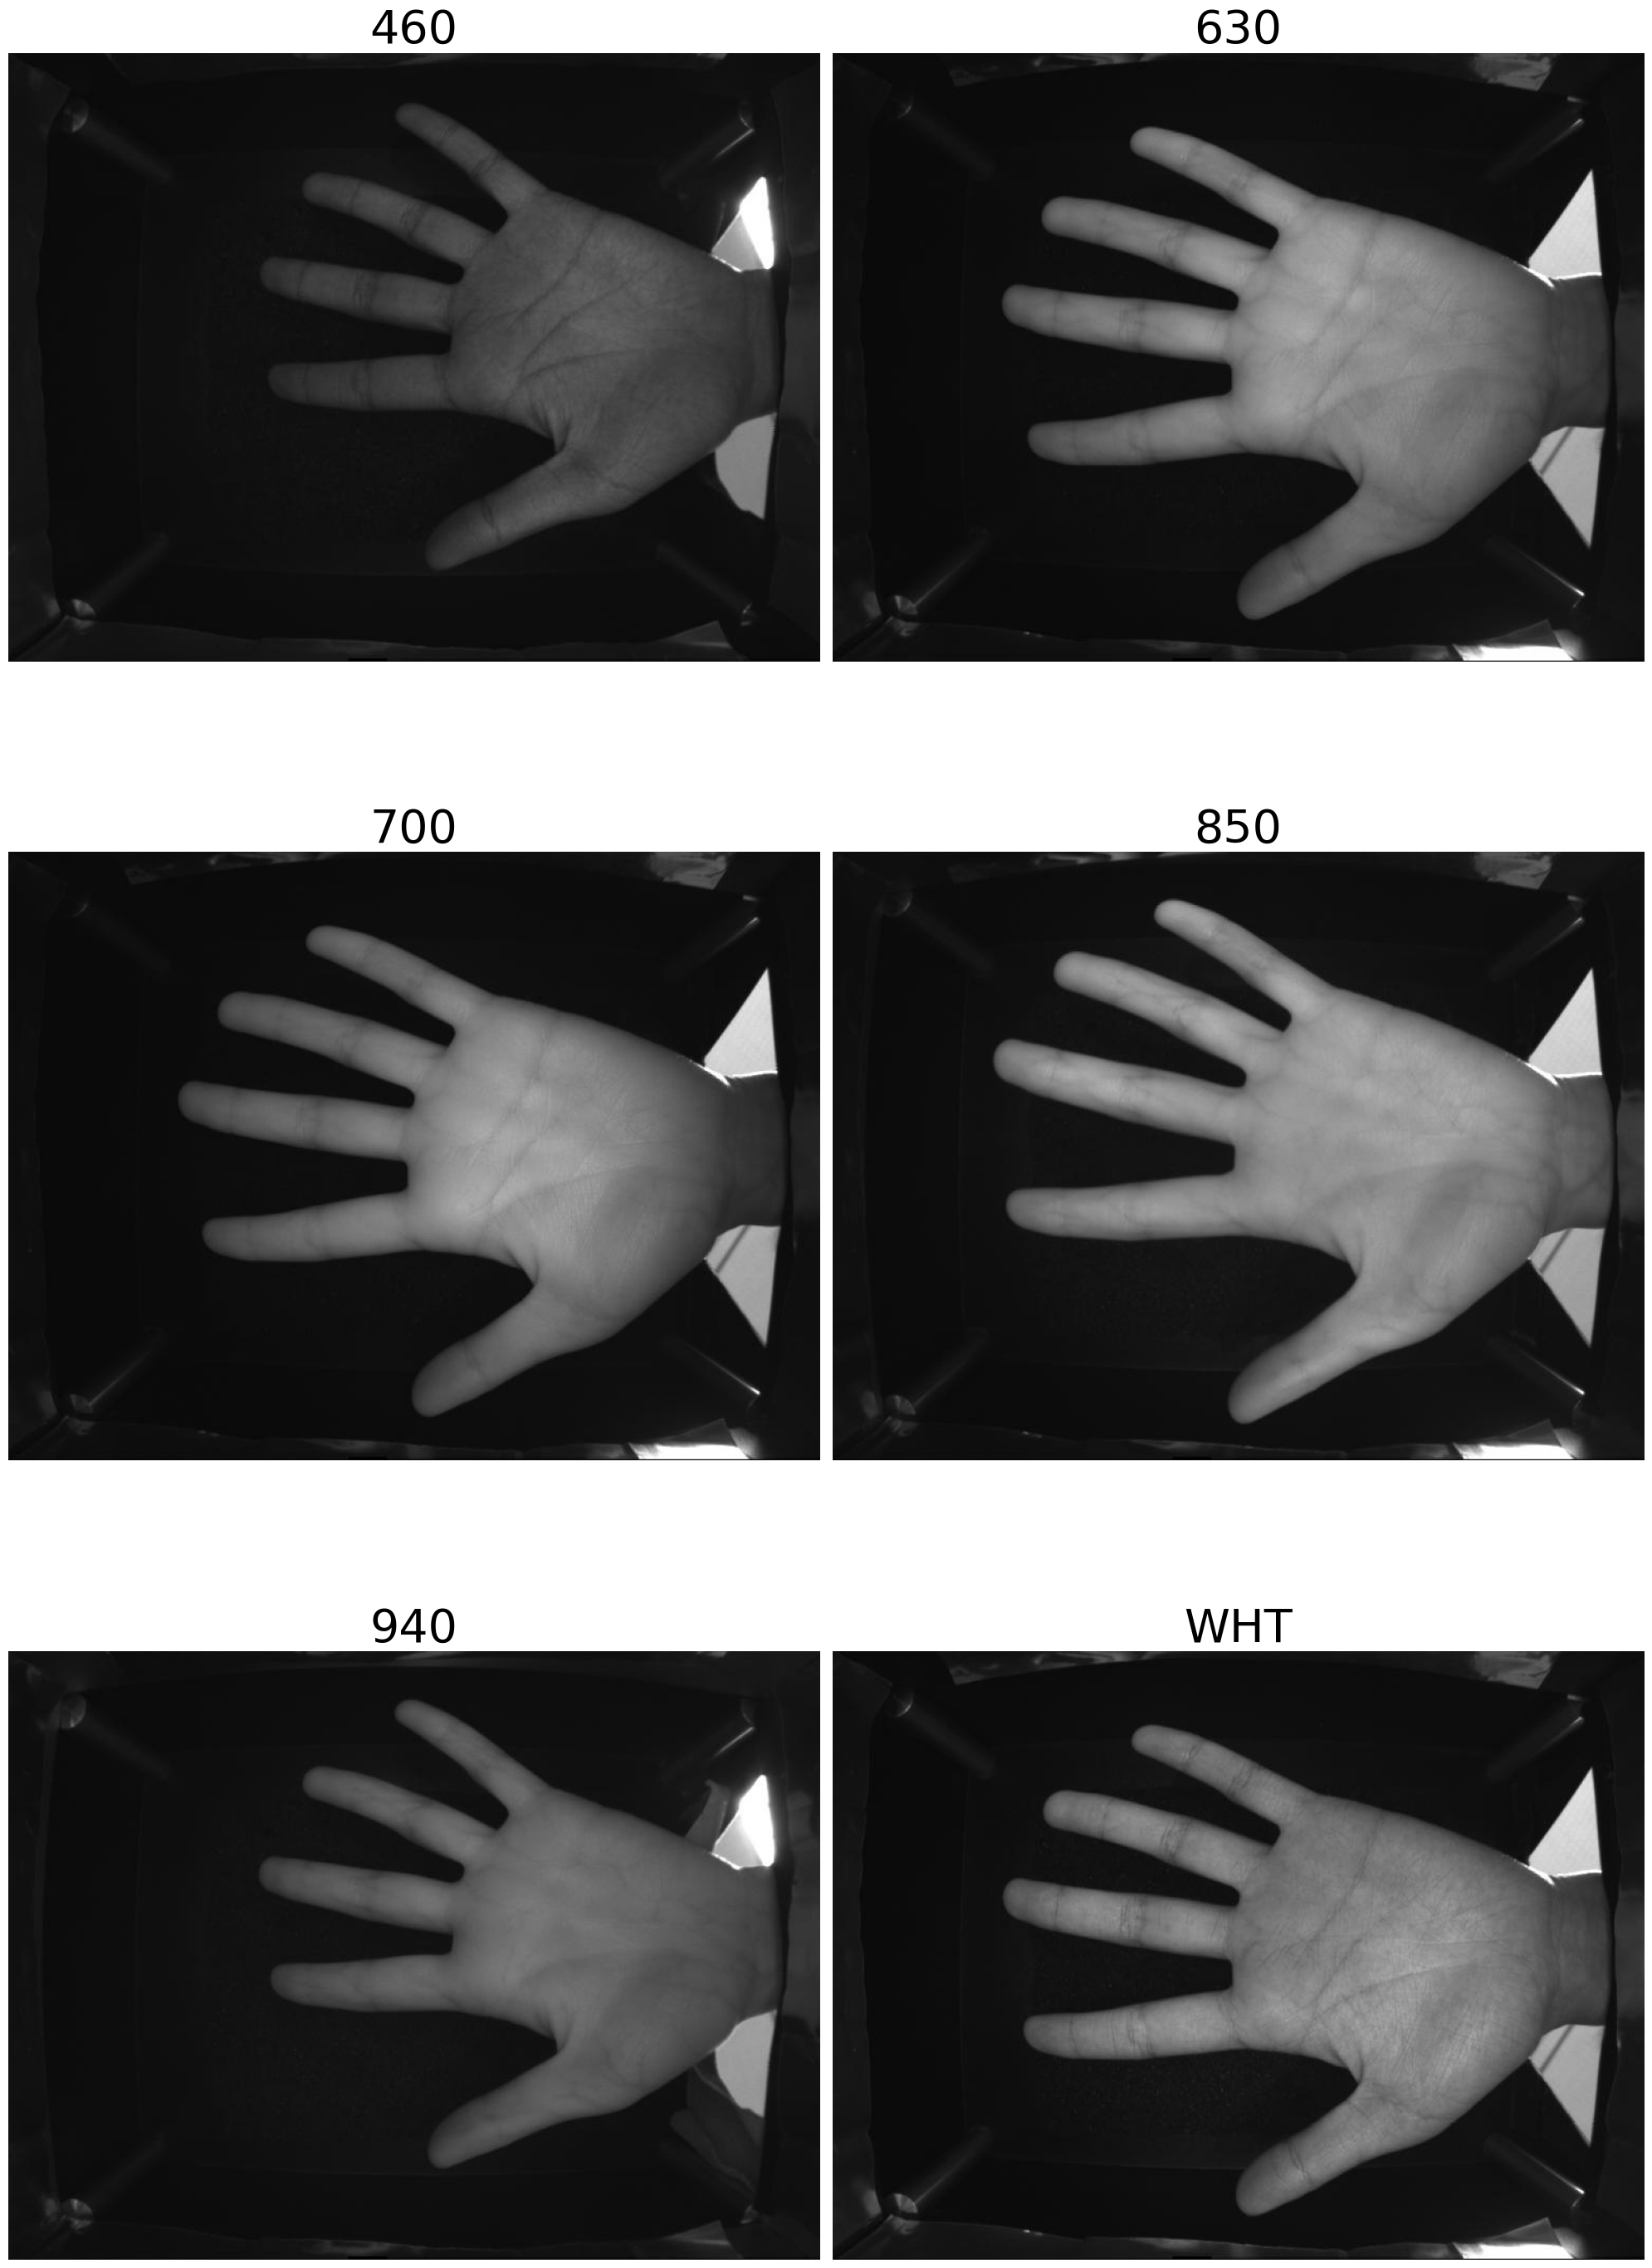
\includegraphics[width=0.3\textwidth]{./images/spectrums.png}
    \caption{Palmprint images from the CASIA Multi-Spectral Palmprint Image Database with the six spectral bands. Starting from the top-left corner and moving clockwise: 460 nm, 630 nm, 700 nm, 850 nm, 940 nm, and white light.}
    \label{fig:dataset_example}
\end{figure}